\documentclass{article}
\usepackage{bbm}
\usepackage{grffile}
\usepackage[utf8]{inputenc}
\usepackage{amsmath,amsfonts,amssymb,amsthm,latexsym,epsfig,epstopdf,titling,url,array}
\usepackage{listings}
\usepackage[normalem]{ulem}
\usepackage{float}
\usepackage{graphicx}
\usepackage{enumerate}

\title{\Huge Creating a Lattice Boltzmann Fluid Solver in TensorFlow}
\author{Vikram Singh}
\date{July 2019}

\setlength{\parindent}{0pt}
\addtolength{\oddsidemargin}{-0.75in}
\addtolength{\evensidemargin}{-0.75in}
\addtolength{\textwidth}{1.5in}

\addtolength{\topmargin}{-0.75in}
\addtolength{\textheight}{1in}

\begin{document}

\maketitle

\section{The Lattice Boltzmann Method}

The Navier-Stokes equations for viscous flow are very complicated, and impossible to solve analytically in many situations. Thus in order to analyse fluid flow in irregular systems, we have to use numerical solvers. One such method is the Lattice Boltzmann Method \cite{wikiLB}. This involves simulating the fluid as populations of particles moving on a discrete lattice with discrete velocities, and simulating collisions at each lattice point. The full method is detailed in \cite{LBBook}.

\section{Potential advantages of TensorFlow}

Many of the operations performed by a Lattice Boltzmann solver are done across large arrays. TensorFlow is used extensively in Machine Learning because of its efficient implementation of operations like this, that are less expensive in time and space than those implemented in Numpy. This efficiency could be used to improve the speed of a Lattice Boltzmann solver. In particular, the calculation of macroscopic variables, and the collision with an obstacle, can be expressed as convolutions of an array, which is implemented very well in TensorFlow. I did some experiments to investigate the potential improvements that TensorFlow could give.

\section{Analysis}

To analyze the benefits of TensorFlow in a solver, I performed some tests using solvers I wrote using both TensorFlow and only Numpy. My code for these solvers is available at (\url{https://github.com/vikram8128/PythonLatticeBoltzmann}).



\subsection{Methodology}

My tests consisted of 6 different simulations, created in both TensorFlow and Numpy versions. These were:

\begin{enumerate}
    \item Flow around a cylinder with low viscosity ($420\times180$)
    \item Flow around a cylinder with high viscosity ($420\times180$)
    \item Flow around an airfoil ($420\times180$)
    \item Flow through a narrowing pipe ($420\times180$)
    \item Flow through a bending pipe ($1000\times452$)
    \item flow in a lid driven cavity ($180\times180$)
\end{enumerate}

The simulations ran for 20000 timesteps, producing .png output every 100 timesteps. Each of these simulations was run on an Intel Skylake server, with access to 32 CPU cores.

\subsection{Results}

The simulations were run 3 times each, and the mean real times are shown in Table 1. 

\begin{table}[H]
\caption{The wallclock times in seconds taken by each simulation}
\begin{center}
\begin{tabular}{c||c|c|c|c|c|c}
\emph{Simulation} & 1 & 2 & 3 & 4 & 5 & 6\\
\hline
\hline
\emph{Numpy} & 316 & 311 & 319 & 1565 & 4043 & 615 \\
\hline
\emph{TensorFlow} & 198 & 198 & 198 & 199 & 708 & 122 \\
\hline
\end{tabular}
\end{center}
\end{table}

In these results, I assumed a generous 10\% uncertainty in the time (observed error was around 2\%). From this, I created the plot in figure 1.

\begin{figure}[H] 
	\centering
	\label{graph}
	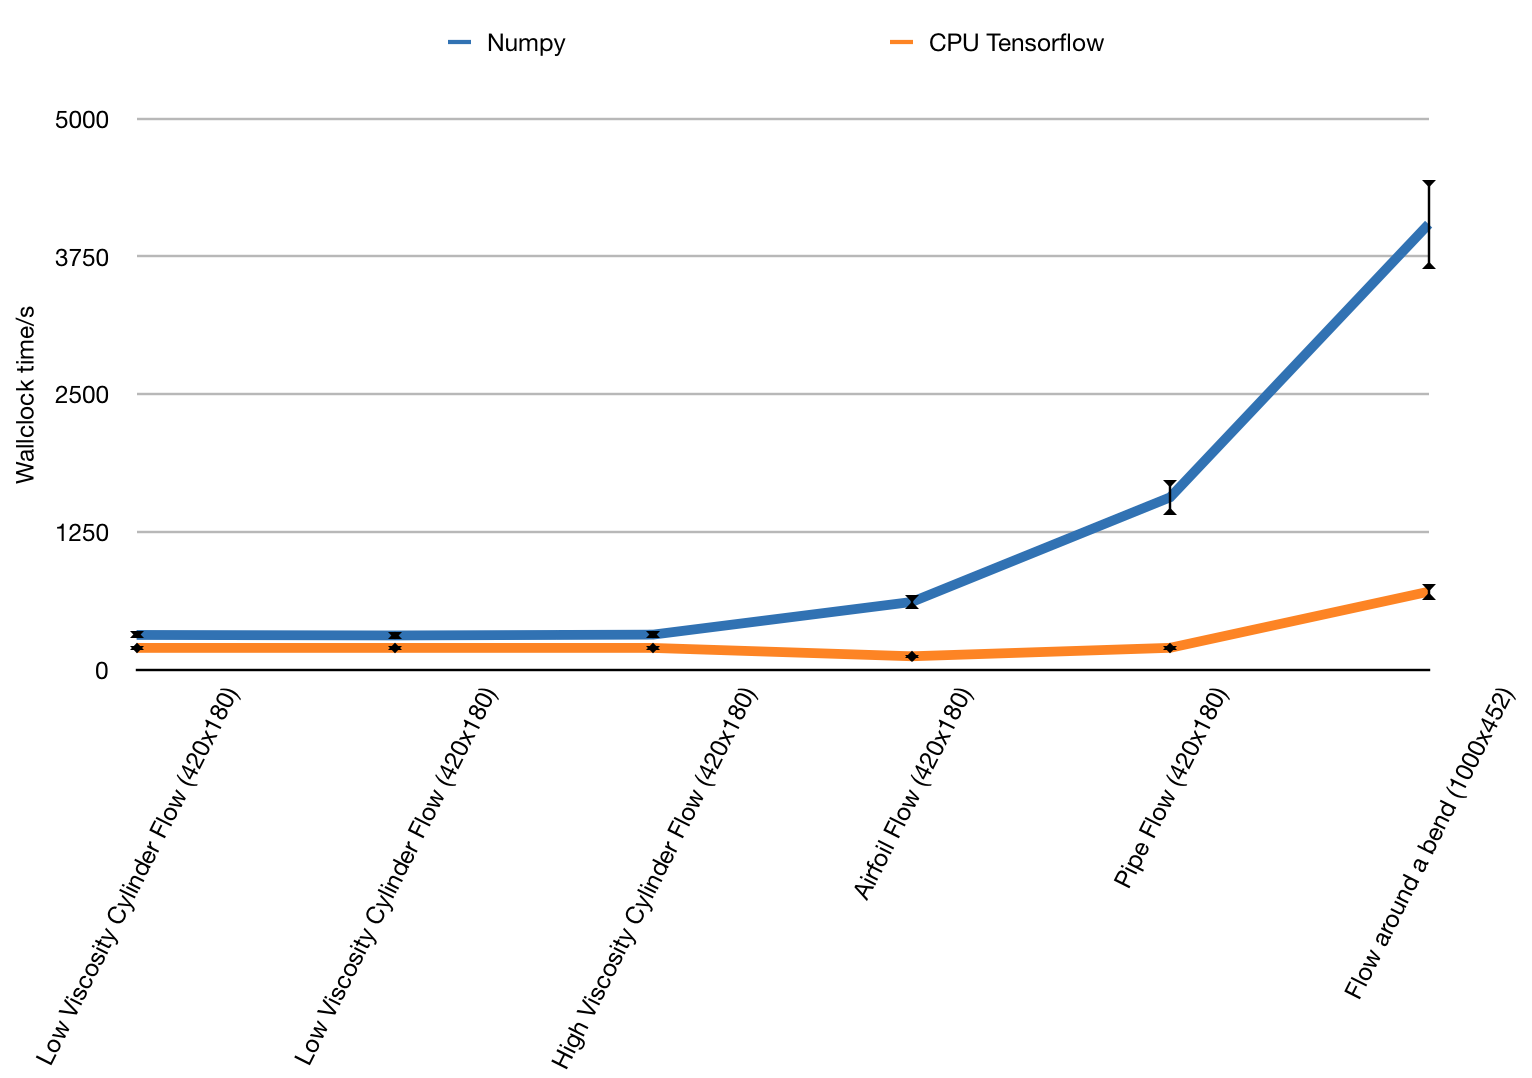
\includegraphics[width=5in]{Diagrams/TimeGraph.png}
	\caption{Runtimes of simulations}
\end{figure}

In addition, I calculated the rate of cell updates (in Megahertz) for each of the simulations, which is shown in table 2.

\begin{table}[H]
\caption{Cell updates per second (MHz) for each of the simulations}
\begin{center}
\begin{tabular}{c||c|c|c|c|c|c}
\emph{Simulation} & 1 & 2 & 3 & 4 & 5 & 6\\
\hline
\hline
\emph{Numpy} & 4.78 & 4.86 & 4.74 & 0.966 & 2.24 & 1.05 \\
\hline
\emph{TensorFlow} & 7.64 & 7.64 & 7.64 & 7.60 & 12.8 & 5.31 \\
\hline
\end{tabular}
\end{center}
\end{table}

Again assuming 10\% uncertainty in this data, we get the plot of cell update frequency in figure 2.

\begin{figure}[H] 
	\centering
	\label{graph}
	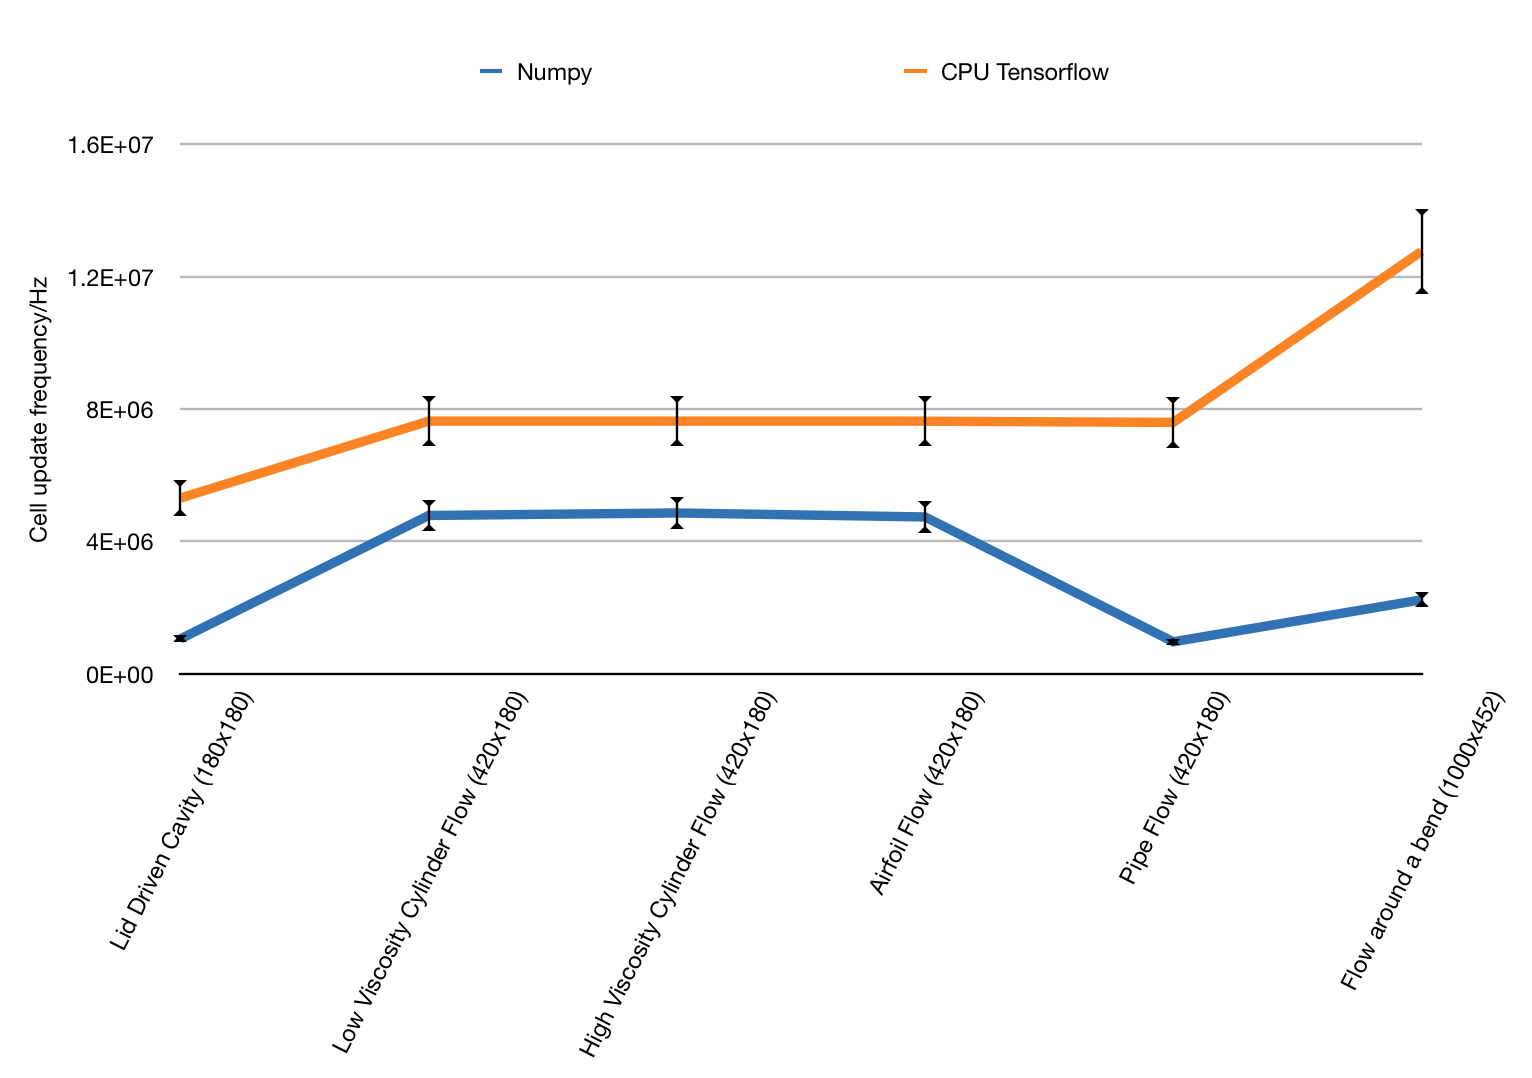
\includegraphics[width=5in]{Diagrams/FreqGraph.png}
	\caption{Cell update frequencies of the simulations}
\end{figure}

\subsection{Conclusions}

We observe that TensorFlow consistently outperforms Numpy, but the improvement factor is not constant. In the simulations of flow in a narrowing pipe, flow in a lid driven cavity and flow in a bending pipe, TensorFlow is faster by a factor of about 5 times, as opposed to about 1.5 in the other three simulations. These simulations have much larger areas of obstacle, and in addition, the bending pipe simulation has a much larger lattice. We can conclude that TensorFlow scales much better than Numpy with an increased lattice size, and an increased area of obstacle. The improved parallelisation that is implemented in TensorFlow gives a large improvement in speed of the Solver, which scales well with size. This improvement could be quite useful for industrial fluid dynamics simulations.

\section{Next Steps}

While this project has provided some useful results, there are some areas that it has not explored. I did not explore how the performance of the models translates to 3D models, where the factor of improvement that TensorFlow provides could be different to the 2D simulations that I examined. Additionally, I only used CPUs to run my TensorFlow simulations. Adapting them slightly to run on GPUs may give a further speed improvement. However, GPU TensorFlow does not support the (\emph{roll}) operation that is used extensively, so this would have to be implemented manually. Both expanding the solvers to 3D, and running the TensorFlow solvers on GPUs would be potentially quite informative, and these require further investigation.

\addcontentsline{toc}{section}{References}
\begin{thebibliography}{99}

\bibitem{wikiLB} Wikipedia article on the Lattice Boltzmann method (\url{en.wikipedia.org/wiki/Lattice_Boltzmann_methods})

\bibitem{LBBook} Alexander J. Wagner (2008) \emph{A Practical Introduction to the Lattice Boltzmann Method}, North Dakota State University

\bibitem{TFDocs} TensorFlow Documentation (\url{www.tensorflow.org/api_docs/python/})

\end{thebibliography}

\end{document}